\documentclass[]{article}
\usepackage{lmodern}
\usepackage{amssymb,amsmath}
\usepackage{ifxetex,ifluatex}
\usepackage{fixltx2e} % provides \textsubscript
\ifnum 0\ifxetex 1\fi\ifluatex 1\fi=0 % if pdftex
  \usepackage[T1]{fontenc}
  \usepackage[utf8]{inputenc}
\else % if luatex or xelatex
  \ifxetex
    \usepackage{mathspec}
  \else
    \usepackage{fontspec}
  \fi
  \defaultfontfeatures{Ligatures=TeX,Scale=MatchLowercase}
\fi
% use upquote if available, for straight quotes in verbatim environments
\IfFileExists{upquote.sty}{\usepackage{upquote}}{}
% use microtype if available
\IfFileExists{microtype.sty}{%
\usepackage{microtype}
\UseMicrotypeSet[protrusion]{basicmath} % disable protrusion for tt fonts
}{}
\usepackage[margin=1in]{geometry}
\usepackage{hyperref}
\hypersetup{unicode=true,
            pdftitle={My Shiny Story},
            pdfauthor={Matt Sharkey},
            pdfborder={0 0 0},
            breaklinks=true}
\urlstyle{same}  % don't use monospace font for urls
\usepackage{color}
\usepackage{fancyvrb}
\newcommand{\VerbBar}{|}
\newcommand{\VERB}{\Verb[commandchars=\\\{\}]}
\DefineVerbatimEnvironment{Highlighting}{Verbatim}{commandchars=\\\{\}}
% Add ',fontsize=\small' for more characters per line
\usepackage{framed}
\definecolor{shadecolor}{RGB}{248,248,248}
\newenvironment{Shaded}{\begin{snugshade}}{\end{snugshade}}
\newcommand{\AlertTok}[1]{\textcolor[rgb]{0.94,0.16,0.16}{#1}}
\newcommand{\AnnotationTok}[1]{\textcolor[rgb]{0.56,0.35,0.01}{\textbf{\textit{#1}}}}
\newcommand{\AttributeTok}[1]{\textcolor[rgb]{0.77,0.63,0.00}{#1}}
\newcommand{\BaseNTok}[1]{\textcolor[rgb]{0.00,0.00,0.81}{#1}}
\newcommand{\BuiltInTok}[1]{#1}
\newcommand{\CharTok}[1]{\textcolor[rgb]{0.31,0.60,0.02}{#1}}
\newcommand{\CommentTok}[1]{\textcolor[rgb]{0.56,0.35,0.01}{\textit{#1}}}
\newcommand{\CommentVarTok}[1]{\textcolor[rgb]{0.56,0.35,0.01}{\textbf{\textit{#1}}}}
\newcommand{\ConstantTok}[1]{\textcolor[rgb]{0.00,0.00,0.00}{#1}}
\newcommand{\ControlFlowTok}[1]{\textcolor[rgb]{0.13,0.29,0.53}{\textbf{#1}}}
\newcommand{\DataTypeTok}[1]{\textcolor[rgb]{0.13,0.29,0.53}{#1}}
\newcommand{\DecValTok}[1]{\textcolor[rgb]{0.00,0.00,0.81}{#1}}
\newcommand{\DocumentationTok}[1]{\textcolor[rgb]{0.56,0.35,0.01}{\textbf{\textit{#1}}}}
\newcommand{\ErrorTok}[1]{\textcolor[rgb]{0.64,0.00,0.00}{\textbf{#1}}}
\newcommand{\ExtensionTok}[1]{#1}
\newcommand{\FloatTok}[1]{\textcolor[rgb]{0.00,0.00,0.81}{#1}}
\newcommand{\FunctionTok}[1]{\textcolor[rgb]{0.00,0.00,0.00}{#1}}
\newcommand{\ImportTok}[1]{#1}
\newcommand{\InformationTok}[1]{\textcolor[rgb]{0.56,0.35,0.01}{\textbf{\textit{#1}}}}
\newcommand{\KeywordTok}[1]{\textcolor[rgb]{0.13,0.29,0.53}{\textbf{#1}}}
\newcommand{\NormalTok}[1]{#1}
\newcommand{\OperatorTok}[1]{\textcolor[rgb]{0.81,0.36,0.00}{\textbf{#1}}}
\newcommand{\OtherTok}[1]{\textcolor[rgb]{0.56,0.35,0.01}{#1}}
\newcommand{\PreprocessorTok}[1]{\textcolor[rgb]{0.56,0.35,0.01}{\textit{#1}}}
\newcommand{\RegionMarkerTok}[1]{#1}
\newcommand{\SpecialCharTok}[1]{\textcolor[rgb]{0.00,0.00,0.00}{#1}}
\newcommand{\SpecialStringTok}[1]{\textcolor[rgb]{0.31,0.60,0.02}{#1}}
\newcommand{\StringTok}[1]{\textcolor[rgb]{0.31,0.60,0.02}{#1}}
\newcommand{\VariableTok}[1]{\textcolor[rgb]{0.00,0.00,0.00}{#1}}
\newcommand{\VerbatimStringTok}[1]{\textcolor[rgb]{0.31,0.60,0.02}{#1}}
\newcommand{\WarningTok}[1]{\textcolor[rgb]{0.56,0.35,0.01}{\textbf{\textit{#1}}}}
\usepackage{longtable,booktabs}
\usepackage{graphicx,grffile}
\makeatletter
\def\maxwidth{\ifdim\Gin@nat@width>\linewidth\linewidth\else\Gin@nat@width\fi}
\def\maxheight{\ifdim\Gin@nat@height>\textheight\textheight\else\Gin@nat@height\fi}
\makeatother
% Scale images if necessary, so that they will not overflow the page
% margins by default, and it is still possible to overwrite the defaults
% using explicit options in \includegraphics[width, height, ...]{}
\setkeys{Gin}{width=\maxwidth,height=\maxheight,keepaspectratio}
\IfFileExists{parskip.sty}{%
\usepackage{parskip}
}{% else
\setlength{\parindent}{0pt}
\setlength{\parskip}{6pt plus 2pt minus 1pt}
}
\setlength{\emergencystretch}{3em}  % prevent overfull lines
\providecommand{\tightlist}{%
  \setlength{\itemsep}{0pt}\setlength{\parskip}{0pt}}
\setcounter{secnumdepth}{0}
% Redefines (sub)paragraphs to behave more like sections
\ifx\paragraph\undefined\else
\let\oldparagraph\paragraph
\renewcommand{\paragraph}[1]{\oldparagraph{#1}\mbox{}}
\fi
\ifx\subparagraph\undefined\else
\let\oldsubparagraph\subparagraph
\renewcommand{\subparagraph}[1]{\oldsubparagraph{#1}\mbox{}}
\fi

%%% Use protect on footnotes to avoid problems with footnotes in titles
\let\rmarkdownfootnote\footnote%
\def\footnote{\protect\rmarkdownfootnote}

%%% Change title format to be more compact
\usepackage{titling}

% Create subtitle command for use in maketitle
\providecommand{\subtitle}[1]{
  \posttitle{
    \begin{center}\large#1\end{center}
    }
}

\setlength{\droptitle}{-2em}

  \title{My Shiny Story}
    \pretitle{\vspace{\droptitle}\centering\huge}
  \posttitle{\par}
    \author{Matt Sharkey}
    \preauthor{\centering\large\emph}
  \postauthor{\par}
      \predate{\centering\large\emph}
  \postdate{\par}
    \date{8/6/2019}


\begin{document}
\maketitle

\hypertarget{from-it-to-data-science}{%
\subsection{From IT to Data Science}\label{from-it-to-data-science}}

At my previous employer, I worked in IT operations as a Database
Administrator. In March of 2018, a colleague on the Data Science team
approached me about an internal job posting. His team was looking for a
Data Engineer to support its data pipeline. I had already worked with
the team on an IT project and few support tickets, so I had an
approximate idea of what skills they needed. I was about to graduate
with a Masters in Analytics, and the opportunity seemed relevant. After
thinking things over, I decided the best route forward was to take the
job.

A team member resigned a few weeks after I signed on. I took on some of
his projects, including the development of a web-app. I had barely
changed my email signature before I started getting feature requests on
the app. I couldn't speak to the feasibility of the requests because I
didn't have experience in the application stack. In fact, I didn't have
much web-app experience in general as I've been a database specialist my
entire career. After several discussions with stakeholders, I pressed
the reset button.

\hypertarget{r-you-serious}{%
\subsection{R you serious?}\label{r-you-serious}}

I decided to re-write the app using R with a SQL Server back-end. At
that point, I had hundreds of hours of R coding experience from grad
school and side projects. Also, most of my coworkers were Data
Scientists and had strong R programming skills. If I had any gaps in my
knowledge, they could help.

The Shiny package in R generates about 95\% of the HTML, CSS, and
JavaScript needed to build a web-app. For example, if I wanted ``Hello
World!'' to appear in the browser, I would have needed to declare it
inside of \textless{}h2\textgreater{} tags. However, with Shiny I called
the h2() function.

\begin{Shaded}
\begin{Highlighting}[]
\OperatorTok{<}\NormalTok{h2}\OperatorTok{>}\NormalTok{Hello World}\OperatorTok{!}\ErrorTok{</}\NormalTok{h2}\OperatorTok{>}
\end{Highlighting}
\end{Shaded}

Hello World!

\begin{Shaded}
\begin{Highlighting}[]
\KeywordTok{library}\NormalTok{(shiny)}

\KeywordTok{h2}\NormalTok{(}\StringTok{'Hello World!'}\NormalTok{)}
\end{Highlighting}
\end{Shaded}

Hello World!

This code generates a date input control.

\begin{Shaded}
\begin{Highlighting}[]
\KeywordTok{dateRangeInput}\NormalTok{(}\StringTok{"date"}\NormalTok{,}
               \KeywordTok{strong}\NormalTok{(}\StringTok{"Date range"}\NormalTok{),}
               \DataTypeTok{start =} \StringTok{"2007-01-01"}\NormalTok{,}
               \DataTypeTok{end =} \StringTok{"2017-07-31"}\NormalTok{,}
               \DataTypeTok{min =} \StringTok{"2007-01-01"}\NormalTok{,}
               \DataTypeTok{max =} \StringTok{"2017-07-31"}
\NormalTok{               )}
\end{Highlighting}
\end{Shaded}

Here's the generated HTML.

\begin{Shaded}
\begin{Highlighting}[]
\OperatorTok{<}\NormalTok{div id=}\StringTok{"date"}\OperatorTok{>}
\ErrorTok{<}\NormalTok{label class=}\StringTok{"control-label"} \ControlFlowTok{for}\NormalTok{=}\StringTok{"date"}\OperatorTok{>}\StringTok{ }\ErrorTok{<}\NormalTok{strong}\OperatorTok{>}\NormalTok{Date range}\OperatorTok{<}\ErrorTok{/}\NormalTok{strong}\OperatorTok{>}
\ErrorTok{</}\NormalTok{label}\OperatorTok{>}\ErrorTok{<}\NormalTok{div class=}\StringTok{"input-daterange input-group"}\OperatorTok{>}
\ErrorTok{<}\NormalTok{input class=}\StringTok{"input-sm form-control"}\NormalTok{ type=}\StringTok{"text"}
\NormalTok{data}\OperatorTok{-}\NormalTok{date}\OperatorTok{-}\NormalTok{week}\OperatorTok{-}\NormalTok{start=}\StringTok{"0"}\NormalTok{ data}\OperatorTok{-}\NormalTok{date}\OperatorTok{-}\NormalTok{format=}\StringTok{"yyyy-mm-dd"}
\NormalTok{data}\OperatorTok{-}\NormalTok{date}\OperatorTok{-}\NormalTok{start}\OperatorTok{-}\NormalTok{view=}\StringTok{"month"}\NormalTok{ data}\OperatorTok{-}\NormalTok{min}\OperatorTok{-}\NormalTok{date=}\StringTok{"2007-01-01"}
\NormalTok{data}\OperatorTok{-}\NormalTok{max}\OperatorTok{-}\NormalTok{date=}\StringTok{"2017-07-31"}\NormalTok{data}\OperatorTok{-}\NormalTok{initial}\OperatorTok{-}\NormalTok{date=}\StringTok{"2007-01-01"}
\NormalTok{data}\OperatorTok{-}\NormalTok{date}\OperatorTok{-}\NormalTok{autoclose=}\StringTok{"true"}\OperatorTok{/}\ErrorTok{><}\NormalTok{span class=}\StringTok{"input-group-addon"}\OperatorTok{>}
\NormalTok{to }\OperatorTok{<}\ErrorTok{/}\NormalTok{span}\OperatorTok{>}\StringTok{ }\ErrorTok{<}\NormalTok{input  type=}\StringTok{"text"}\NormalTok{ data}\OperatorTok{-}\NormalTok{date}\OperatorTok{-}\NormalTok{language=}\StringTok{"en"}
\NormalTok{data}\OperatorTok{-}\NormalTok{date}\OperatorTok{-}\NormalTok{week}\OperatorTok{-}\NormalTok{start=}\StringTok{"0"}\NormalTok{ data}\OperatorTok{-}\NormalTok{date}\OperatorTok{-}\NormalTok{format=}\StringTok{"yyyy-mm-dd"}
\NormalTok{data}\OperatorTok{-}\NormalTok{min}\OperatorTok{-}\NormalTok{date=}\StringTok{"2007-01-01"}\NormalTok{ data}\OperatorTok{-}\NormalTok{max}\OperatorTok{-}\NormalTok{date=}\StringTok{"2017-07-31"}\OperatorTok{/}\ErrorTok{>}
\StringTok{  }\ErrorTok{</}\NormalTok{div}\OperatorTok{>}\ErrorTok{</}\NormalTok{div}\OperatorTok{>}
\end{Highlighting}
\end{Shaded}

\hypertarget{the-game-plan}{%
\subsection{The Game Plan}\label{the-game-plan}}

My strategy was to push as much logic and data processing to the
database as possible. I felt this was the best route because, again,
most of my experience is on the database side. I also had concerns about
R performance. R by default runs on one thread whereas SQL server by
default can multi-thread.

I knew code generators were great for productivity but often at the cost
of performance and functionality. It wasn't clear to me how the app
would handle database connections, application errors, or perform with
multiple user sessions. As I progressed on the project, I learned a few
techniques that put those concerns to rest. It's my goal in this post to
share those techniques.

\hypertarget{app-architecture}{%
\subsection{App Architecture}\label{app-architecture}}

Before we can start discussing performance tuning, we must establish the
basics. The main components of my Shiny app are UI, the Server object,
and the database.

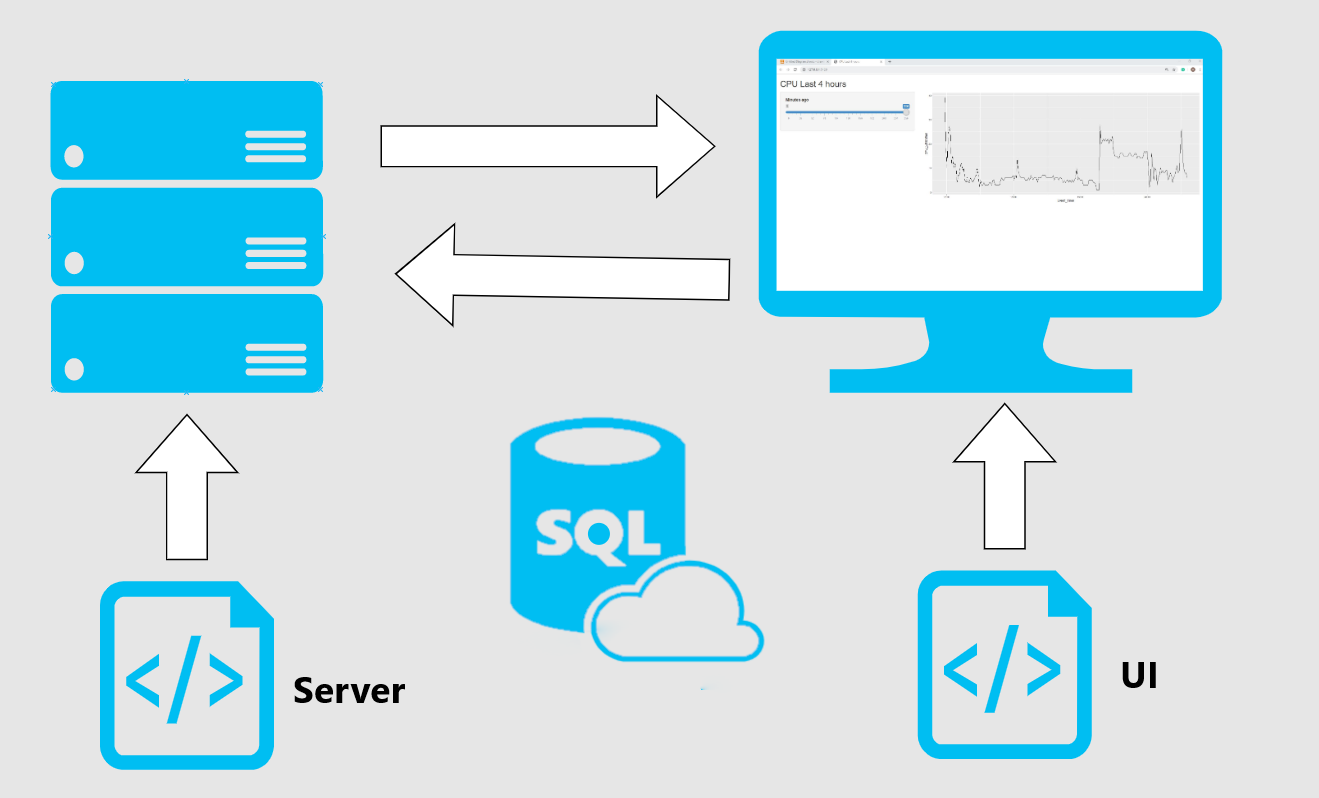
\includegraphics{./Images/ShinyArc.png}

The code below provides the base components required for a Shiny
database app. Multiple projects can use this template as a starting
point.

\begin{Shaded}
\begin{Highlighting}[]
\KeywordTok{library}\NormalTok{(shiny)}
\KeywordTok{library}\NormalTok{(DBI)}
\KeywordTok{library}\NormalTok{(odbc)}

\NormalTok{con <-}\StringTok{ }\KeywordTok{dbConnect}\NormalTok{(}\DataTypeTok{drv =} \KeywordTok{odbc}\NormalTok{(),  }\DataTypeTok{Driver =} \StringTok{'Sql Server'}\NormalTok{,}\DataTypeTok{Server =} \StringTok{'.}\CharTok{\textbackslash{}\textbackslash{}}\StringTok{snapman'}\NormalTok{,}\DataTypeTok{Database =} \StringTok{'Test'}\NormalTok{)}

\NormalTok{my_ui <-}\StringTok{ }\KeywordTok{fluidPage}\NormalTok{()}
 
\NormalTok{my_server <-}\StringTok{ }\ControlFlowTok{function}\NormalTok{(input, output) \{\}}

\KeywordTok{shinyApp}\NormalTok{(}\DataTypeTok{ui =}\NormalTok{ my_ui, }\DataTypeTok{server =}\NormalTok{ my_server)}
\end{Highlighting}
\end{Shaded}

\hypertarget{ui}{%
\subsubsection{UI}\label{ui}}

The date input control above is one of many components in the UI. The UI
also contains formatting, theme data, and server outputs like graphs.

The image below shows what the completed UI looks like for a sample app.
The app has two UI components- a slider control and a plot displaying
CPU utilization over time.

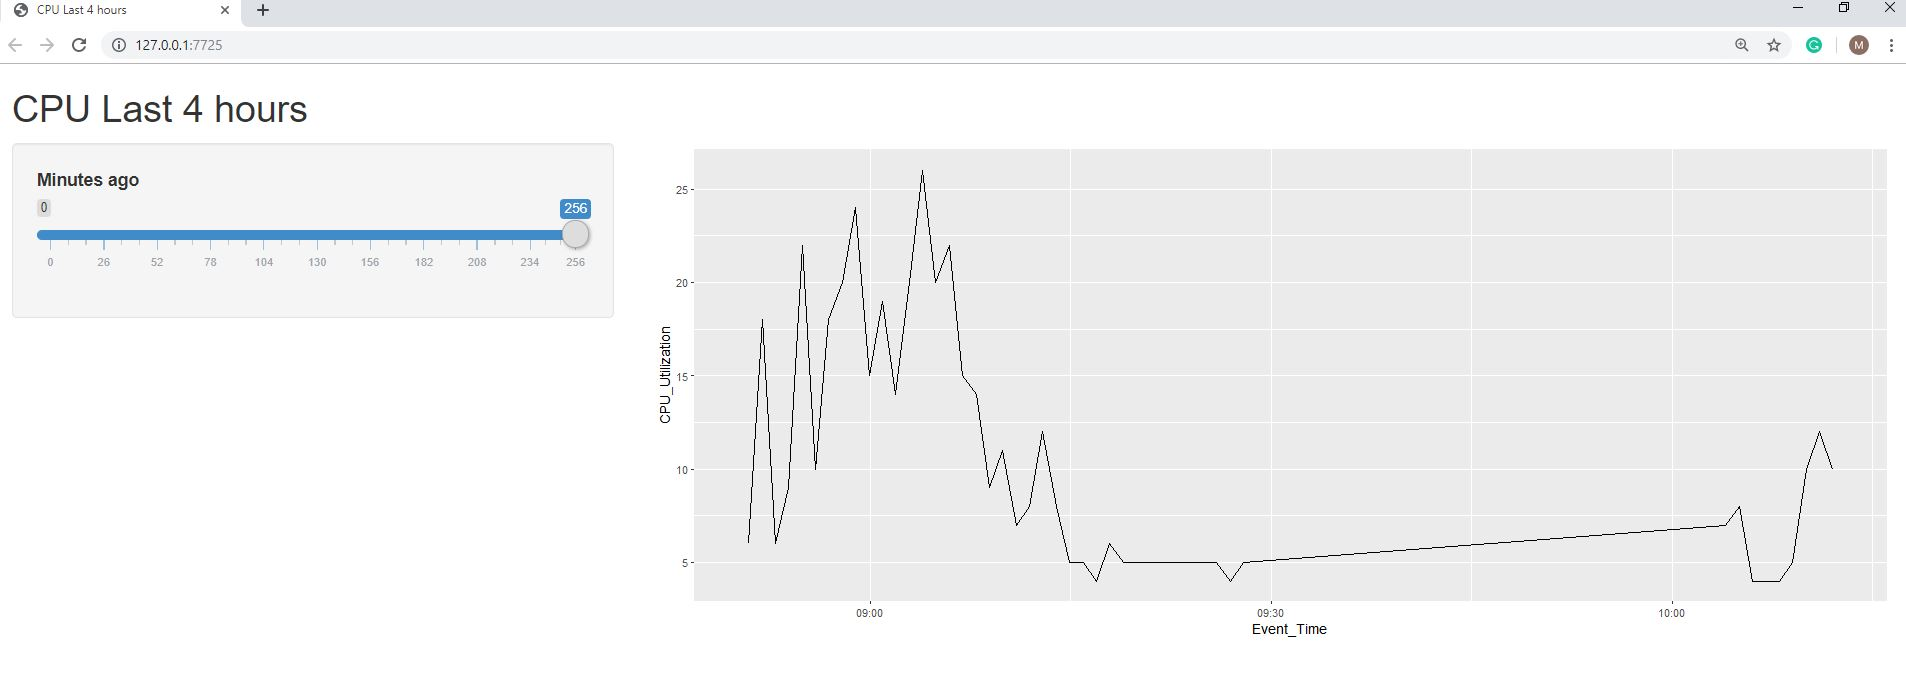
\includegraphics{./Images/BaseApp.JPG}

The slider helps users determine how far back the plot should display
data up to a max of the last 256 minutes. We create the slider with the
sliderinput() function. It's important to note that the value for input
Id must be unique for each input object because we reference it in the
server object. The server object wouldn't know which input to accept if
we had duplicate input Ids. Finally, we wrap the slider in a sidebar to
give the page an organized look.

\begin{Shaded}
\begin{Highlighting}[]
\KeywordTok{library}\NormalTok{(shiny)}

\NormalTok{con <-}\StringTok{ }\KeywordTok{dbConnect}\NormalTok{(}\DataTypeTok{drv =} \KeywordTok{odbc}\NormalTok{(),  }\DataTypeTok{Driver =} \StringTok{'Sql Server'}\NormalTok{,}\DataTypeTok{Server =} \StringTok{'.}\CharTok{\textbackslash{}\textbackslash{}}\StringTok{snapman'}\NormalTok{,}\DataTypeTok{Database =} \StringTok{'Test'}\NormalTok{)}

\NormalTok{my_ui <-}\StringTok{ }\KeywordTok{fluidPage}\NormalTok{(}\KeywordTok{sidebarPanel}\NormalTok{(}\KeywordTok{sliderInput}\NormalTok{(}\StringTok{"cpu_slider"}\NormalTok{,}\StringTok{"Minutes Back"}\NormalTok{,}\DecValTok{0}\NormalTok{,}\DecValTok{256}\NormalTok{,}\DecValTok{256}\NormalTok{))}

\NormalTok{my_server <-}\StringTok{ }\ControlFlowTok{function}\NormalTok{(input, output) \{\}}

\KeywordTok{shinyApp}\NormalTok{(}\DataTypeTok{ui =}\NormalTok{ my_ui, }\DataTypeTok{server =}\NormalTok{ my_server)}
\end{Highlighting}
\end{Shaded}

Now we need to add a function for our plot. The plotOutput() currently
references a plot called ``cpuPlot.'' cpuPlot does not exist, so the
main panel is nothing but a placeholder at the moment.

\begin{Shaded}
\begin{Highlighting}[]
\KeywordTok{library}\NormalTok{(shiny)}

\NormalTok{con <-}\StringTok{ }\KeywordTok{dbConnect}\NormalTok{(}\DataTypeTok{drv =} \KeywordTok{odbc}\NormalTok{(),  }\DataTypeTok{Driver =} \StringTok{'Sql Server'}\NormalTok{,}\DataTypeTok{Server =} \StringTok{'.}\CharTok{\textbackslash{}\textbackslash{}}\StringTok{snapman'}\NormalTok{,}\DataTypeTok{Database =} \StringTok{'Test'}\NormalTok{)}

\NormalTok{my_ui <-}\StringTok{ }\KeywordTok{fluidPage}\NormalTok{(}\KeywordTok{sidebarPanel}\NormalTok{(}\KeywordTok{sliderInput}\NormalTok{(}\StringTok{"cpu_slider"}\NormalTok{,}\StringTok{"Minutes Back"}\NormalTok{,}\DecValTok{0}\NormalTok{,}\DecValTok{256}\NormalTok{,}\DecValTok{256}\NormalTok{))}
\NormalTok{                   , }\KeywordTok{mainPanel}\NormalTok{(}\KeywordTok{plotOutput}\NormalTok{(}\StringTok{"cpuPlot"}\NormalTok{)))}

\NormalTok{my_server <-}\StringTok{ }\ControlFlowTok{function}\NormalTok{(input, output) \{\}}

\KeywordTok{shinyApp}\NormalTok{(}\DataTypeTok{ui =}\NormalTok{ my_ui, }\DataTypeTok{server =}\NormalTok{ my_server)}
\end{Highlighting}
\end{Shaded}

\hypertarget{server-and-database-integration}{%
\subsection{Server and Database
Integration}\label{server-and-database-integration}}

The server object renders plots and returns them to UI. The plot uses a
stored procedure based on a Glen Berry SQL Server monitoring query.
There are numerous benefits of using stored procs, and I'll touch on a
few. First, stored means logic lives server-side instead of inline on
the front-end. We can change the app logic on the database without
having to take down the app. Second, I can grant permissions to execute
the stored procedure without granting permissions on the underlying
tables. A security best practice is to grant access to interfaces and
not implementations. Tables are implementations, and stored procedures
are interfaces. Finally, stored procs reduce the query string length,
which means less data transferred for each execution. For high volume
systems, the savings can add up.

\begin{Shaded}
\begin{Highlighting}[]

\KeywordTok{CREATE} \KeywordTok{OR} \KeywordTok{ALTER} \KeywordTok{PROCEDURE}\NormalTok{ dbo.GetCPUutilization}
\OtherTok{@minutes INT = 256}
\KeywordTok{AS}
\KeywordTok{SET}\NormalTok{ NOCOUNT }\KeywordTok{ON}
\KeywordTok{DECLARE}\NormalTok{ @ts_now BIGINT }\OperatorTok{=}\NormalTok{ (}
            \KeywordTok{SELECT}\NormalTok{ cpu_ticks }\OperatorTok{/}\NormalTok{ (cpu_ticks }\OperatorTok{/}\NormalTok{ ms_ticks)}
              \KeywordTok{FROM}\NormalTok{ sys.dm_os_sys_info }\KeywordTok{WITH}\NormalTok{ (NOLOCK)}
\NormalTok{        );}

\KeywordTok{SELECT}\NormalTok{ TOP (}\DecValTok{256}\NormalTok{) DATEADD(ms, }\OperatorTok{-}\DecValTok{1} \OperatorTok{*}\NormalTok{ (@ts_now }\OperatorTok{-}\NormalTok{ [}\DataTypeTok{timestamp}\NormalTok{]), GETDATE()) }\KeywordTok{AS}\NormalTok{ [Event_Time],}
                 \DecValTok{100} \OperatorTok{-}\NormalTok{ SystemIdle                                     }\KeywordTok{AS}\NormalTok{ [CPU_Utilization]}
  \KeywordTok{FROM}\NormalTok{ (}
      \KeywordTok{SELECT} 
\DataTypeTok{record}\NormalTok{.}\FunctionTok{value}\NormalTok{(}\StringTok{'(./Record/@id)[1]'}\NormalTok{, }\StringTok{'int'}\NormalTok{) }\KeywordTok{AS}\NormalTok{ record_id,}
\DataTypeTok{record}\NormalTok{.}\FunctionTok{value}\NormalTok{(}\StringTok{'(./Record/SchedulerMonitorEvent/SystemHealth/SystemIdle)[1]'}
\NormalTok{, }\StringTok{'int'}\NormalTok{)         }\KeywordTok{AS}\NormalTok{ [SystemIdle],}
\DataTypeTok{record}\NormalTok{.}\FunctionTok{value}\NormalTok{(}\StringTok{'(./Record/SchedulerMonitorEvent/SystemHealth/ProcessUtilization)[1]'}
\NormalTok{, }\StringTok{'int'}\NormalTok{) }\KeywordTok{AS}\NormalTok{ [SQLProcessUtilization],}
\NormalTok{[}\DataTypeTok{timestamp}\NormalTok{]}
        \KeywordTok{FROM}\NormalTok{ (}
            \KeywordTok{SELECT}\NormalTok{ [}\DataTypeTok{timestamp}\NormalTok{],}
                   \FunctionTok{CONVERT}\NormalTok{(XML, }\DataTypeTok{record}\NormalTok{) }\KeywordTok{AS}\NormalTok{ [}\DataTypeTok{record}\NormalTok{]}
              \KeywordTok{FROM}\NormalTok{ sys.dm_os_ring_buffers }\KeywordTok{WITH}\NormalTok{ (NOLOCK)}
             \KeywordTok{WHERE}\NormalTok{ ring_buffer_type }\OperatorTok{=}\NormalTok{ N}\StringTok{'RING_BUFFER_SCHEDULER_MONITOR'}
               \KeywordTok{AND} \DataTypeTok{record} \KeywordTok{LIKE}\NormalTok{ N}\StringTok{'%<SystemHealth>%'}
\NormalTok{        ) }\KeywordTok{AS}\NormalTok{ x}
\NormalTok{  ) }\KeywordTok{AS}\NormalTok{ y}
  \KeywordTok{WHERE}\NormalTok{ DATEADD(ms, }\OperatorTok{-}\DecValTok{1} \OperatorTok{*}\NormalTok{ (@ts_now }\OperatorTok{-}\NormalTok{ [}\DataTypeTok{timestamp}\NormalTok{]), GETDATE()) }\OperatorTok{>=}\NormalTok{ DateAdd(}\KeywordTok{minute}\NormalTok{,}\OperatorTok{-}\NormalTok{@minutes,Getdate())}
 \KeywordTok{ORDER} \KeywordTok{BY}\NormalTok{ record_id }\KeywordTok{DESC}
\KeywordTok{OPTION}\NormalTok{ (RECOMPILE);}

\NormalTok{GO}
\end{Highlighting}
\end{Shaded}

\begin{Shaded}
\begin{Highlighting}[]
\KeywordTok{EXECUTE}\NormalTok{ dbo.GetCPUutilization}
\end{Highlighting}
\end{Shaded}

\begin{longtable}[]{@{}lr@{}}
\caption{Displaying records 1 - 10}\tabularnewline
\toprule
Event\_Time & CPU\_Utilization\tabularnewline
\midrule
\endfirsthead
\toprule
Event\_Time & CPU\_Utilization\tabularnewline
\midrule
\endhead
2019-08-10 10:22:24 & 13\tabularnewline
2019-08-10 10:21:24 & 11\tabularnewline
2019-08-10 10:20:24 & 16\tabularnewline
2019-08-10 10:19:24 & 18\tabularnewline
2019-08-10 10:18:24 & 8\tabularnewline
2019-08-10 10:17:24 & 19\tabularnewline
2019-08-10 10:16:24 & 16\tabularnewline
2019-08-10 10:15:24 & 16\tabularnewline
2019-08-10 10:14:24 & 16\tabularnewline
2019-08-10 10:13:24 & 7\tabularnewline
\bottomrule
\end{longtable}

So now our app can execute a stored procedure by referencing it in a
dbGetQuery call.

\begin{Shaded}
\begin{Highlighting}[]
\KeywordTok{library}\NormalTok{(odbc)}
\KeywordTok{library}\NormalTok{(DBI)}

\NormalTok{my_ui <-}\StringTok{ }\KeywordTok{fluidPage}\NormalTok{(}\KeywordTok{sidebarPanel}\NormalTok{(}\KeywordTok{sliderInput}\NormalTok{(}\StringTok{"cpu_slider"}\NormalTok{,}\StringTok{"Minutes Back"}\NormalTok{,}\DecValTok{0}\NormalTok{,}\DecValTok{256}\NormalTok{,}\DecValTok{256}\NormalTok{))}
\NormalTok{                   , }\KeywordTok{mainPanel}\NormalTok{(}\KeywordTok{plotOutput}\NormalTok{(}\StringTok{"cpuPlot"}\NormalTok{)))}

\NormalTok{my_server <-}\StringTok{ }\ControlFlowTok{function}\NormalTok{(input, output) \{}
\NormalTok{  output}\OperatorTok{$}\NormalTok{cpuPlot <-}\StringTok{ }\KeywordTok{renderPlot}\NormalTok{(\{}
\NormalTok{  con <-}\StringTok{ }\KeywordTok{dbConnect}\NormalTok{(}\DataTypeTok{drv =} \KeywordTok{odbc}\NormalTok{(),  }\DataTypeTok{Driver =} \StringTok{'Sql Server'}\NormalTok{,}\DataTypeTok{Server =} \StringTok{'.}\CharTok{\textbackslash{}\textbackslash{}}\StringTok{snapman'}\NormalTok{,}\DataTypeTok{Database =} \StringTok{'Test'}\NormalTok{)}
\NormalTok{  myquery <-}\StringTok{ "EXECUTE dbo.GetCPUutilization"}
\NormalTok{  mydata <-}\StringTok{ }\KeywordTok{dbGetQuery}\NormalTok{(con,myquery)}

    \KeywordTok{dbDisconnect}\NormalTok{(con)}
\end{Highlighting}
\end{Shaded}

We want users to filter the time frame with the slider input. We should
filter the results as soon as possible. In this case, that means adding
a predicate to the WHERE clause. The WHERE clause contains a stored
procedure parameter. R can pass values to that parameter in the myquery
string.

The input control modifies the query string for each user interaction.
dbGetQuery executes the code and stores the result set to mydata. Next,
my data passes the data to ggplot() which generates the plot. Finally,
the updated contents of out\$cpuplot render to the UI.

\begin{Shaded}
\begin{Highlighting}[]
\KeywordTok{library}\NormalTok{(odbc)}
\KeywordTok{library}\NormalTok{(DBI)}

\NormalTok{my_ui <-}\StringTok{ }\KeywordTok{fluidPage}\NormalTok{(}\KeywordTok{sidebarPanel}\NormalTok{(}\KeywordTok{sliderInput}\NormalTok{(}\StringTok{"cpu_slider"}\NormalTok{,}\StringTok{"Minutes Back"}\NormalTok{,}\DecValTok{0}\NormalTok{,}\DecValTok{256}\NormalTok{,}\DecValTok{256}\NormalTok{))}
\NormalTok{                   , }\KeywordTok{mainPanel}\NormalTok{(}\KeywordTok{plotOutput}\NormalTok{(}\StringTok{"cpuPlot"}\NormalTok{)))}

\NormalTok{my_server <-}\StringTok{ }\ControlFlowTok{function}\NormalTok{(input, output) \{}

\NormalTok{  output}\OperatorTok{$}\NormalTok{cpuPlot <-}\StringTok{ }\KeywordTok{renderPlot}\NormalTok{(\{}
\NormalTok{  con <-}\StringTok{ }\KeywordTok{dbConnect}\NormalTok{(}\DataTypeTok{drv =} \KeywordTok{odbc}\NormalTok{(),}
                   \DataTypeTok{Driver =} \StringTok{'Sql Server'}\NormalTok{,}\DataTypeTok{Server =} \StringTok{'.}\CharTok{\textbackslash{}\textbackslash{}}\StringTok{snapman'}\NormalTok{,}\DataTypeTok{Database =} \StringTok{'Test'}\NormalTok{ )}
\NormalTok{  myquery <-}\StringTok{ }\KeywordTok{paste0}\NormalTok{(}\StringTok{"Execute dbo.getCPUutilization "}\NormalTok{,input}\OperatorTok{$}\NormalTok{cpu_slider)}

\NormalTok{mydata <-}\StringTok{ }\KeywordTok{dbGetQuery}\NormalTok{(con,myquery)}

\KeywordTok{dbDisconnect}\NormalTok{(con)}
 \KeywordTok{ggplot}\NormalTok{(mydata,}\KeywordTok{aes}\NormalTok{(Event_Time,CPU_Utilization)) }\OperatorTok{+}\StringTok{ }\KeywordTok{geom_line}\NormalTok{()}
\NormalTok{  \})}

\NormalTok{\}}

\KeywordTok{shinyApp}\NormalTok{(}\DataTypeTok{ui =}\NormalTok{ my_ui, }\DataTypeTok{server =}\NormalTok{ my_server)}
\end{Highlighting}
\end{Shaded}

We now have a basic app! It needs a little work before it is
production-ready.

\hypertarget{security}{%
\subsubsection{Security}\label{security}}

A pressing security issue is concatenating user input with the query
string. As a rule of thumb, never mix trusted data (in this case, the
query string) with untrusted data (the user input). If a user passed a
string for the input, then they could execute arbitrary commands against
the database. Put another way; the app is vulnerable to injection
attacks. Parameterization reduces the risk of injection attacks by
separating trusted data (the query) with untrusted data (user input).
The sqlinterpolate function from DBI implements parametrization. With
the change, the user cannot modify the query string at runtime.

\begin{Shaded}
\begin{Highlighting}[]
\NormalTok{myquery <-}\StringTok{ "EXECUTE dbo.getCPUutilization ?cpu_slider_param"}

\NormalTok{myquery_param <-}\StringTok{ }\KeywordTok{sqlInterpolate}\NormalTok{(con,myquery,}\DataTypeTok{.dots =}\KeywordTok{c}\NormalTok{(cpu_slider_param <-}\StringTok{ }\NormalTok{input}\OperatorTok{$}\NormalTok{cpu_slider))}

\NormalTok{mydata <-}\StringTok{ }\KeywordTok{dbGetQuery}\NormalTok{(con,myquery_param)}
\end{Highlighting}
\end{Shaded}

It's a good idea to validate inputs with whitelists. For example, check
that an email input field follows a specified pattern. The code below
populates emailistwhitelist with a regex pattern of a valid email. The
if() function checks if the input matches the pattern. If it doesn't
match, then query won't touch the database.

\begin{Shaded}
\begin{Highlighting}[]
\NormalTok{emailwhitelist <-}\StringTok{ "^[[:alnum:].-_]+@[[:alnum:].-]+$"}

\ControlFlowTok{if}\NormalTok{(}\OperatorTok{!}\KeywordTok{is.na}\NormalTok{(}\KeywordTok{str_match}\NormalTok{(usr_email, emailwhitelist)))\{}
  \CommentTok{#Run query}
\NormalTok{\} }\ControlFlowTok{else}
\NormalTok{\{}
  \CommentTok{# Reject input}
\NormalTok{\}}
\end{Highlighting}
\end{Shaded}

\hypertarget{connection-management}{%
\subsubsection{Connection Management}\label{connection-management}}

The app seems a little sluggish. If performance isn't acceptable, then
the first place to turn is profvis. Profvis provides line by line
execution metrics for R code. The profvis function launches the app.
Then we interact with the application as an average user would. When the
browser closes, profvis generates a report with a .Rprofvis extension.
The report shows memory consumed and execution time for each function.
Also, a flame graph shows execution time at each stage of the call
stack.

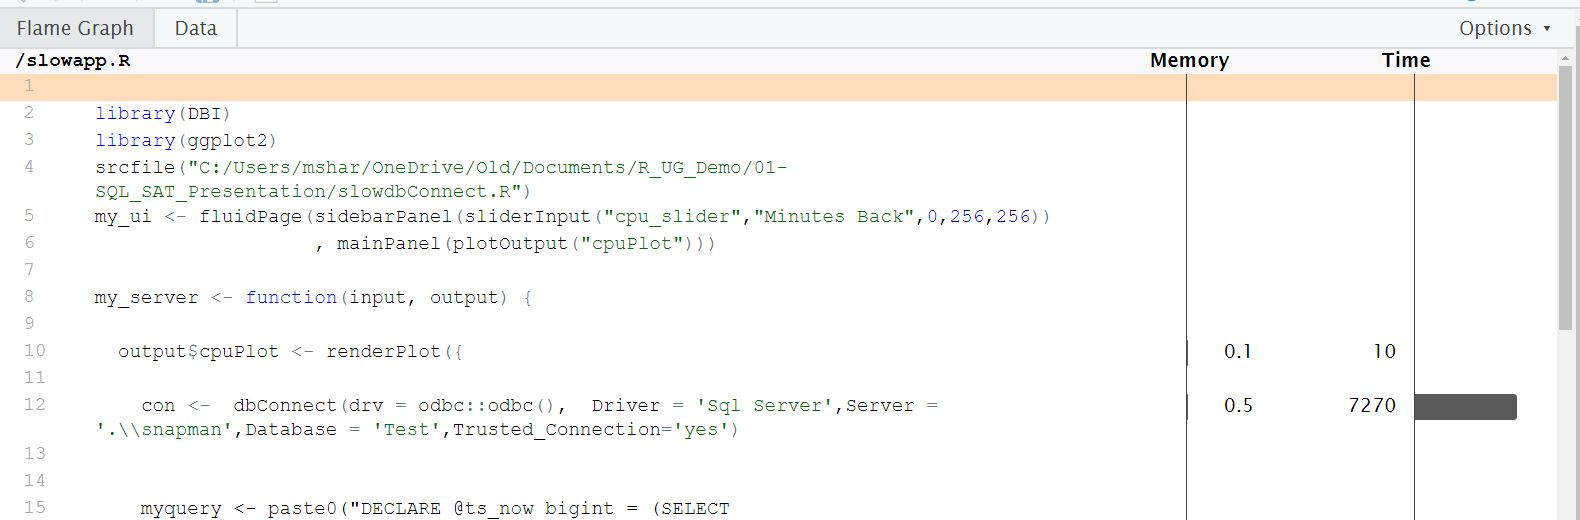
\includegraphics{./Images/ProfvisData.JPG}

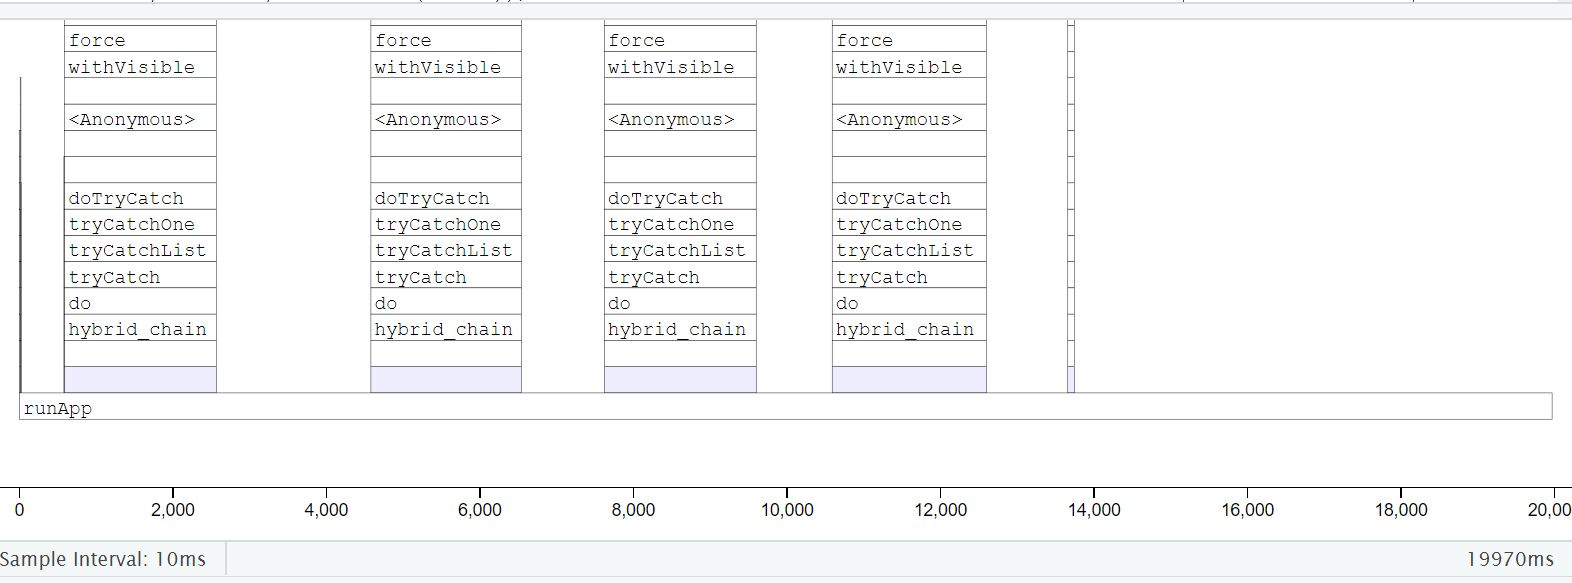
\includegraphics{./Images/Flame.JPG}

The profile session reveals dbConnect() accounts for most of the
execution time. The app makes a connection to our database each time the
user adjusts the slider input. Instead of opening and closing a
connection for each query, we could grab an open connection from a pool.
The pool library allows us to use pooling with a few code changes. First
we replace the dbConnect() with dbPool(). We don't need to close the
pool when the application is running so dbDisconnect() gets removed.
Finally, we move dbPool() outside of the server object completely.

\begin{Shaded}
\begin{Highlighting}[]
\KeywordTok{library}\NormalTok{(pool)}
\NormalTok{pool <-}\StringTok{ }\KeywordTok{dbPool}\NormalTok{(}\DataTypeTok{drv =} \KeywordTok{odbc}\NormalTok{(),}\DataTypeTok{Driver =}\NormalTok{ mydriver,}\DataTypeTok{Server =}\NormalTok{ myserver,}\DataTypeTok{Database =}\NormalTok{ myDatabase)}
\NormalTok{  results <-}\StringTok{ }\KeywordTok{dbGetQuery}\NormalTok{(pool,myquery)}
\end{Highlighting}
\end{Shaded}

Besides making our session faster, pool also helps the app scale. Pool
opens and closes connections as needed without developer intervention.
So as the workload starts to increase more open connection become
available.

\hypertarget{error-handling}{%
\subsubsection{Error Handling}\label{error-handling}}

Error handling can improve user experience and prevent the app from
crashing. If an error occurs, the app should do something like alert the
user. When we increase app complexity, we increase the need for error
handling. Adding a relational database to the app is an example of
increasing complexity. It's a good idea to build redundancy around the
database connection. How would the app respond if the database server
went down? How would the app respond if there was a deadlock? I'll
simulate a database outage by forcing the database offline while the app
is running.

\begin{Shaded}
\begin{Highlighting}[]
\KeywordTok{ALTER} \KeywordTok{Database}\NormalTok{ Test }\KeywordTok{Set}\NormalTok{ SINGLE_USER }\KeywordTok{WITH} \KeywordTok{ROLLBACK} \KeywordTok{IMMEDIATE}\NormalTok{;}
\KeywordTok{ALTER} \KeywordTok{Database}\NormalTok{ Test }\KeywordTok{Set} \KeywordTok{OFFLINE}\NormalTok{;}
\end{Highlighting}
\end{Shaded}

When the user adjusts the slider, the query attempts to re-run but
fails. R displays an error containing the query text where the plot
should be. This error is not helpful to the average user. Also, the app
shouldn't expose implementation details like table names to end-users.

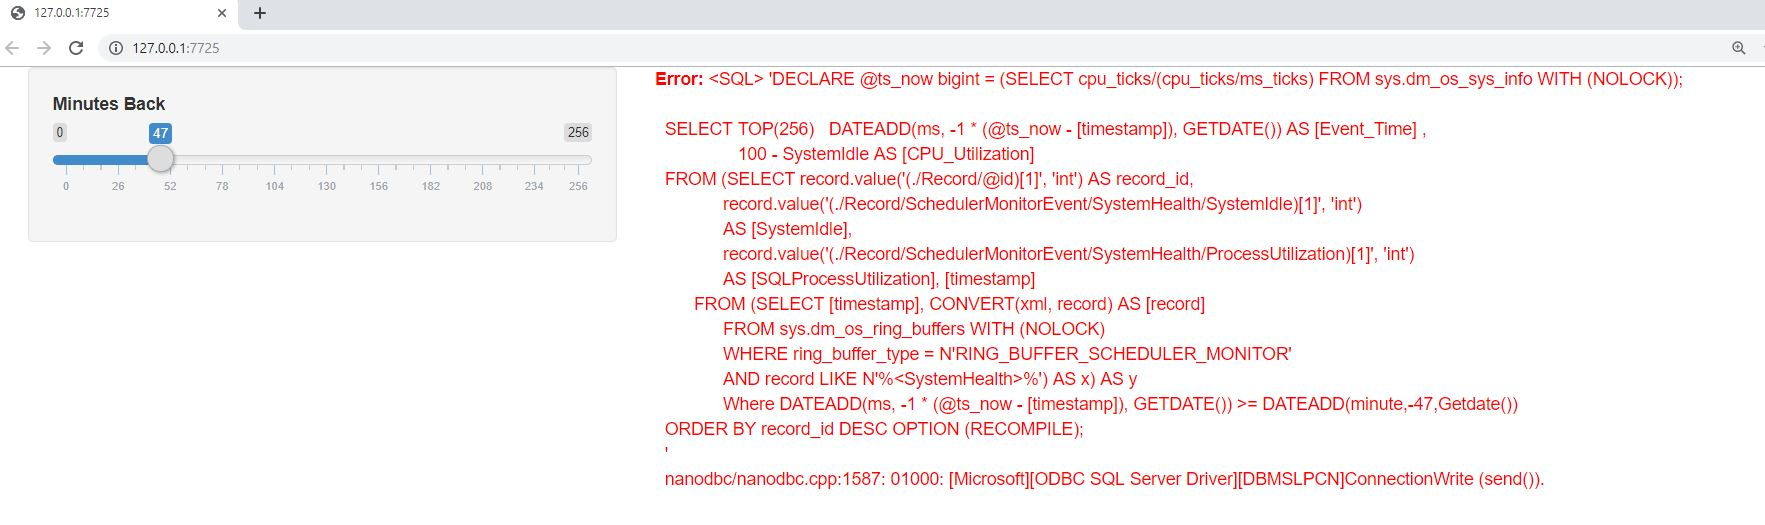
\includegraphics{./Images/ErrorMessage.JPG}

We can avoid this issue with a tryCatch function wrapped around the
query execution. If an error occurs, code in the error function
executes.

\begin{Shaded}
\begin{Highlighting}[]
      \KeywordTok{tryCatch}\NormalTok{(\{}
\NormalTok{        results <-}\StringTok{ }\KeywordTok{dbGetQuery}\NormalTok{(pool,myquery)}
\NormalTok{        j<-}\StringTok{ }\KeywordTok{ggplot}\NormalTok{(results,}\KeywordTok{aes}\NormalTok{(Event_Time,CPU_Utilization))}
\NormalTok{        j}\OperatorTok{+}\StringTok{ }\KeywordTok{geom_line}\NormalTok{()}
\NormalTok{        \},}\DataTypeTok{error =}\ControlFlowTok{function}\NormalTok{(e) \{}
            \KeywordTok{showModal}\NormalTok{(}\KeywordTok{modalDialog}\NormalTok{(}
                \KeywordTok{h5}\NormalTok{(}\StringTok{'There was an error.  Please contact the system admin.'}\NormalTok{)}
\NormalTok{            )}
\NormalTok{            )}
\NormalTok{        \})}
\end{Highlighting}
\end{Shaded}

Now instead of red error messages, the user gets a modal box with
instructions.

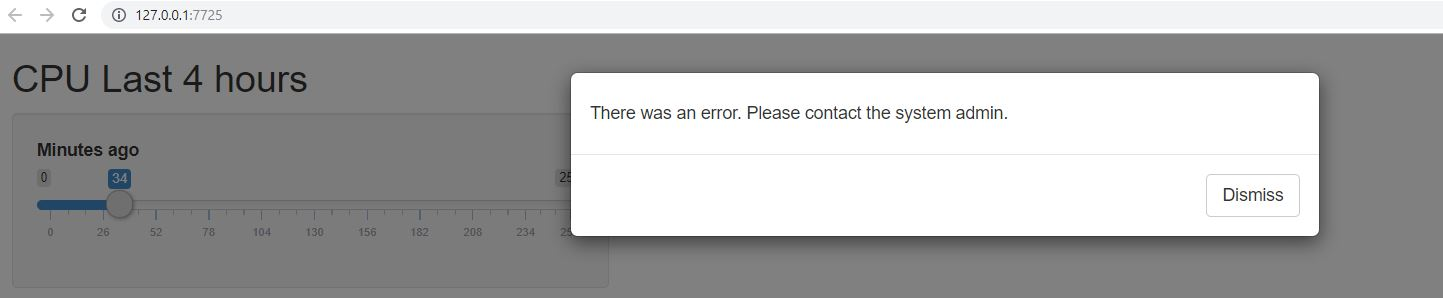
\includegraphics{./Images/ModalError.JPG}

The error function stores error details from the R session like the
error message. It's possible to write error specific messages or events.
For example, we could retry the query if the text contains ``1205'' in
the error text. SQL server throws 1205 errors when it detects deadlocks.
R retries three times before giving up.

\begin{Shaded}
\begin{Highlighting}[]
\KeywordTok{tryCatch}\NormalTok{(\{}
    \KeywordTok{dbGetQuery}\NormalTok{(con,myquery)}
\NormalTok{\}}
\NormalTok{,}\DataTypeTok{error =} \ControlFlowTok{function}\NormalTok{(e)\{}
  \ControlFlowTok{if}\NormalTok{(}\KeywordTok{grep}\NormalTok{(}\StringTok{'1205'}\NormalTok{,e}\OperatorTok{$}\NormalTok{message)}\OperatorTok{==}\DecValTok{1}\NormalTok{)\{}
    \ControlFlowTok{while}\NormalTok{ (x}\OperatorTok{<}\DecValTok{4}\NormalTok{)\{}
      \KeywordTok{tryCatch}\NormalTok{(\{}
        \KeywordTok{dbGetQuery}\NormalTok{(con,myquery)}
        \ControlFlowTok{break}
\NormalTok{        \}}
\NormalTok{      ,}\DataTypeTok{error=}\ControlFlowTok{function}\NormalTok{(e)\{}
\NormalTok{      x<<-}\StringTok{ }\NormalTok{x}\OperatorTok{+}\DecValTok{1}
\NormalTok{      \})}
\NormalTok{    \}}
\NormalTok{  \}}
\NormalTok{\})}
\end{Highlighting}
\end{Shaded}

\hypertarget{load-testing}{%
\subsubsection{Load Testing}\label{load-testing}}

The app has reached acceptable performance for one user session. But,
how does the app handle concurrent user sessions? We can find out using
a load test. Load tests depend on the shinyload package, the shinycannon
program, and Java.

The first step of a load test is recording a typical user session. I
record the session with the app hosted on my local machine. I start two
instances of Rstudio. One runs the Shiny app, and the other runs the
recording function record\_session().

\begin{Shaded}
\begin{Highlighting}[]
\NormalTok{shinyloadtest}\OperatorTok{::}\KeywordTok{record_session}\NormalTok{(}\StringTok{'http://127.0.0.1:6696/'}\NormalTok{)}
\end{Highlighting}
\end{Shaded}

The record\_session function launches the app in a browser. Once the
browser closes, Shinycannon writes the session actions to recording.log.
Shinycannon replays recording.log for as long and in as many user
sessions specified. The second required argument is the app URL. We'll
see how the app performs with 50 users for two minutes of load. The
following code runs in a terminal.

\begin{Shaded}
\begin{Highlighting}[]
\ExtensionTok{java}\NormalTok{ -jar shinycannon-1.0.0-c9c02cb.jar recording.log http://127.0.0.1:4978/ --workers 50 --loaded-duration-minutes 2}
\end{Highlighting}
\end{Shaded}

After the load test finishes, we can view the results through
shinyloadtest.

\begin{Shaded}
\begin{Highlighting}[]
\NormalTok{df <-}\StringTok{ }\NormalTok{shinyloadtest}\OperatorTok{::}\KeywordTok{load_runs}\NormalTok{(}\StringTok{"50workers"}\NormalTok{ =}\StringTok{ "./test-logs-2019-07-22T03_21_19.997Z"}\NormalTok{)}

\NormalTok{shinyloadtest}\OperatorTok{::}\KeywordTok{shinyloadtest_report}\NormalTok{(df, }\StringTok{"run1.html"}\NormalTok{)}
\end{Highlighting}
\end{Shaded}

49 48 47 46 45 44 43 42 41 40 39 38 37 36 35 34 33 32 31 30 29 28 27 26
25 24 23 22 21 20 19 18 17 16 15 14 13 12 11 10 9 8 7 6 5 4 3 2 1 0 0 50
100 150 Elapsed time (sec) Simulated User \# Homepage JS/CSS Start
session Calculate Warmup / Cooldown

The X-Axis represents elapsed time, and the Y-axis represents displays
each session. The black dots show the app under full load. Full load in
this specific test means 50 concurrent users. At ten concurrent users,
session performance plummets. The 11th app user would be waiting seconds
for plots to render. Interrupting workflow for this long makes for
unhappy users. We need a go-faster button.

\hypertarget{caching}{%
\subsubsection{Caching}\label{caching}}

We know that two of the most expensive function were renderPlot and
dbGetQuery. We can't tune the query much, but we can remove the
OPTION(recompile) query hint. Removing the hint enables plan caching on
the SQL server. Instead of recompiling the plan each time our app looks
it up in cache.

\begin{Shaded}
\begin{Highlighting}[]
\OperatorTok{--}\KeywordTok{OPTION}\NormalTok{ (RECOMPILE);}\StringTok{"## Disabling hint so plan caching can occur}
\end{Highlighting}
\end{Shaded}

We can also enable plot caching with minor app code changes. First, the
renderCachedPlot function replaces renderPlot. Second, we specify a
cache key after the renderCachedPlot closing curly brace. The natural
choice is the input slider. When a user selects the same input, they, in
theory, would be requesting the same plot. Rather than re-render the
same plot, the app can retrieve it from cache.

\begin{Shaded}
\begin{Highlighting}[]
  \ErrorTok{\}}\NormalTok{,cacheKeyExpr =}\StringTok{ }\NormalTok{\{input}\OperatorTok{$}\NormalTok{cpu_slider\}}\ErrorTok{)}
\end{Highlighting}
\end{Shaded}

Before we re-run the load test, I must point out that our app would not
work with caching in its current state. The query returns a sliding
window and is not deterministic. Say, for example, I submit a query with
a slider input value of 256. Then five minutes later, I submit the same
query. The data would change, but if we pulled the plot from cache, it
would reflect stale data. We could persist the results of the query in a
table and update the input control to a timestamp or numeric field. This
change makes the app compatible with plot caching. For the demo, we do
not add the change as the focus is on performance implications. With
plot caching, the load test reveals a significant performance
enhancement.

49 48 47 46 45 44 43 42 41 40 39 38 37 36 35 34 33 32 31 30 29 28 27 26
25 24 23 22 21 20 19 18 17 16 15 14 13 12 11 10 9 8 7 6 5 4 3 2 1 0 0 50
100 150 Elapsed time (sec) Simulated User \# Homepage JS/CSS Start
session Calculate Warmup / Cooldown

Each event now executes in milliseconds, which improves concurrency. The
50th user has a similar experience with the app as the first. It's a
safe assumption the app can scale beyond 50 users. Here's the completed
app.

\begin{Shaded}
\begin{Highlighting}[]
\KeywordTok{library}\NormalTok{(DBI)}
\KeywordTok{library}\NormalTok{(ggplot2)}
\KeywordTok{library}\NormalTok{(pool)}

\KeywordTok{tryCatch}\NormalTok{(\{}
\NormalTok{con <-}\StringTok{  }\KeywordTok{dbPool}\NormalTok{(}\DataTypeTok{drv =}\NormalTok{ odbc}\OperatorTok{::}\KeywordTok{odbc}\NormalTok{(),}
               \DataTypeTok{Driver =} \StringTok{'Sql Server'}\NormalTok{,}\DataTypeTok{Server =} \StringTok{'.}\CharTok{\textbackslash{}\textbackslash{}}\StringTok{snapman'}\NormalTok{,}\DataTypeTok{Database =} \StringTok{'Test'}\NormalTok{)}
\NormalTok{\},}\DataTypeTok{error =} \ControlFlowTok{function}\NormalTok{(e)\{}\KeywordTok{showModal}\NormalTok{(}\KeywordTok{modalDialog}\NormalTok{(}\StringTok{'Connection Error'}\NormalTok{))\})}

\NormalTok{my_ui <-}\StringTok{ }\KeywordTok{fluidPage}\NormalTok{(}\KeywordTok{sidebarPanel}\NormalTok{(}\KeywordTok{sliderInput}\NormalTok{(}\StringTok{"cpu_slider"}\NormalTok{,}\StringTok{"Minutes Back"}\NormalTok{,}\DecValTok{0}\NormalTok{,}\DecValTok{256}\NormalTok{,}\DecValTok{256}\NormalTok{))}
\NormalTok{                   , }\KeywordTok{mainPanel}\NormalTok{(}\KeywordTok{plotOutput}\NormalTok{(}\StringTok{"cpuPlot"}\NormalTok{)))}

\NormalTok{my_server <-}\StringTok{ }\ControlFlowTok{function}\NormalTok{(input, output) \{}
\NormalTok{  output}\OperatorTok{$}\NormalTok{cpuPlot <-}\StringTok{ }\KeywordTok{renderCachedPlot}\NormalTok{(\{}
\NormalTok{    myquery <-}\StringTok{ }\KeywordTok{paste0}\NormalTok{(}\StringTok{"Execute dbo.getCPUutilization ?minRange"}\NormalTok{)}
\NormalTok{    myqueryint <-}\StringTok{ }\KeywordTok{sqlInterpolate}\NormalTok{(con,myquery,}\DataTypeTok{.dots=}\KeywordTok{c}\NormalTok{(}\DataTypeTok{minRange=}\NormalTok{input}\OperatorTok{$}\NormalTok{cpu_slider))}
    \KeywordTok{tryCatch}\NormalTok{(\{}
\NormalTok{      mydata <-}\StringTok{ }\KeywordTok{dbGetQuery}\NormalTok{(con,myqueryint)}
      \KeywordTok{ggplot}\NormalTok{(mydata,}\KeywordTok{aes}\NormalTok{(Event_Time,CPU_Utilization)) }\OperatorTok{+}\StringTok{ }\KeywordTok{geom_line}\NormalTok{()\},}
      \DataTypeTok{error =} \ControlFlowTok{function}\NormalTok{(e)\{}
        \KeywordTok{showModal}\NormalTok{(}\KeywordTok{modalDialog}\NormalTok{(}\StringTok{'There was an error.'}\NormalTok{))}
\NormalTok{      \}}
\NormalTok{    )}
\NormalTok{  \},}\DataTypeTok{cacheKeyExpr =}\NormalTok{ input}\OperatorTok{$}\NormalTok{cpu_slider)}
\NormalTok{\}}
\KeywordTok{shinyApp}\NormalTok{(}\DataTypeTok{ui =}\NormalTok{ my_ui, }\DataTypeTok{server =}\NormalTok{ my_server)}
\end{Highlighting}
\end{Shaded}

\hypertarget{summary}{%
\subsubsection{Summary}\label{summary}}

At my last job, I took responsibility for a web-app written in an
unfamiliar stack. I re-wrote the app using the R package Shiny, which
helped simplify the development process. I had concerns about scale and
functionality. I learned with proper design; a Shiny app can serve 50
users efficiently. I used R functions for improving security, connection
management, error handling, and caching.

I ended up using Shiny for several other Data Science projects. Each
project had unique requirements and challenges. And each time R had an
answer. If a Data Science team needs to write a self-service web-app,
then R is a solid choice.


\end{document}
